\documentclass{article}
\usepackage{amsmath, amssymb, amsthm}
\usepackage{tikz}
\usepackage{geometry}
\usepackage[T1]{fontenc}
\geometry{margin=1in}

\title{MAIA 1: Topologie i przestrzenie metryczne}
\author{}
\date{}

\begin{document}
\maketitle

\section{Zbiory}
\begin{enumerate}
\item $X$ - przestrzeń/zbiór
\item $A \subseteq X$
\item $A^c = \{x \in X : x \notin A\}$
\item $\emptyset = X^c$ \quad zbiór pusty/podzbioru
\item $2^X$ - rodzina podzbiorów $X$
\end{enumerate}

$A^B \Rightarrow$ wszystkie funkcje $f: B \to A$

\section{Dla $A_\alpha \subset X$}
$\alpha \in I$ (dowolny zbiór indeksów)

$$\bigcup_{\alpha \in I} A_\alpha = \{x \in X: \exists_{\alpha \in I} x \in A_\alpha\}$$

$$\bigcap_{\alpha \in I} A_\alpha = \{x: \forall_{\alpha \in I} x \in A_\alpha\}$$

\section{Dla $A_n \subset X, \; n \in \mathbb{N}, \ldots$}
$$\lim_{n \to \infty} A_n = \limsup_{n} A_n$$

\begin{equation*}
\bigcap_{n=1}^{\infty} \left( \bigcup_{k \geq n} A_k \right)
\end{equation*}

$$\lim_{n \to \infty} A_n = \liminf_{n} A_n$$

\begin{equation*}
\bigcup_{n=1}^{\infty} \left( \bigcap_{k \geq n} A_k \right)
\end{equation*}

\vspace{0.3cm}
\textbf{Fakt:}
\begin{enumerate}
\item $\lim_{n} A_n \subset \liminf_{n} A_n$
\item $\left( \lim_{n} A_n \right)^c = \liminf_{n} A_n^c$
\item $\left( \lim_{n} A_n \right)^c = \liminf_{n} A_n^c$
\end{enumerate}

\textbf{Def:} $\lim_{n} A_n = \lim_{n} A_n \Rightarrow \lim_{n} A_n = \liminf_{n} A_n = \limsup_{n} A_n$

\section{CP}
$A \times B = \{(x,y): x \in A, y \in B \}$

\subsection{Topologia}
\subsubsection{Przestrzeń topo. (X, $\tau$) $\rightarrow$ rodzina podzbiorów w sensie}
\begin{itemize}
\item[(a)] $A_\alpha \in \tau, \; \alpha \in I \Rightarrow \bigcup_{\alpha \in I} A_\alpha \in \tau$
\item[(b)] $A_1, \ldots, A_n \in \tau, \; n \in \mathbb{N} \Rightarrow \bigcap_{k=1}^n A_k \in \tau$
\item[(c)] $\emptyset, X \in \tau$
\end{itemize}

$\tau$ - topologia

$A \in \tau \Rightarrow$ open set\\
closed set: $A^c$

\subsection{Funkcje ciągłe}
given $(X, \tau_1)$, $(Y, \tau_2)$

$f: X \to Y$ jest ciągła iff 
$$\forall_{A \in \tau_2} f^{-1}[A] \in \tau_1$$

$$\{x \in X: f(x) \in A\}$$

\section{Przestrzeń metryczna $(X, d)$}
$d: X \times X \to [0,\infty)$ takie że:

\begin{enumerate}
\item $d(x,y) = 0 \Leftrightarrow x = y$
\item $\forall x, y \in X \quad d(x,y) = d(y,x)$
\item $\forall x, y, z \in X \quad d(x,y) \leq d(x,z) + d(z,y)$
\end{enumerate}

\section{Kula}
Dla $x_0 \in X, \; R > 0$
$$B(x_0, R) = \{x \in X: d(x_0, x) < R\}$$
closed ball, sphere

\section{Zbiór $A \subset X$ jest otwarty w $X$ iff}
$$\forall x \in A \; \exists R > 0 \quad B(x, R) \subset A$$

\textbf{Fakt:} Tak zdef. rodzina zbiorów otwartych jest topologią.

\vspace{0.3cm}
\textit{przykład} $X = \mathbb{R}^2$

$d_0((x_1,y_1), (x_2,y_2)) = \begin{cases} 
0 & \text{if } (x_1,y_1) = (x_2,y_2) \\
1 & \text{otherwise}
\end{cases}$

$d_1$ - Euclidea
$d_2$ - metryka taksówkowa

\section{Przestrzeń liniowa nad ciałem $\mathbb{K}$}
has addition and number defined

$\forall x,y \in X \; \forall \alpha,\beta \in X \quad \alpha x + \beta y \in X$

\section{Przestrzeń unormowana}
$(X, \|\cdot\|) \rightarrow \|\cdot\|: X \to [0,\infty)$

\begin{enumerate}
\item $\|x\| = 0 \Leftrightarrow x = 0$
\item $\forall x \in X \; \forall \alpha \in \mathbb{K} \quad \|\alpha x\| = |\alpha| \cdot \|x\|$
\item $\forall x,y \in X \quad \|x+y\| \leq \|x\| + \|y\|$
\end{enumerate}

\textbf{Fakt:} $d(x,y) = \|x-y\|$ jest metryką na $X$

\vspace{0.3cm}
\textit{przykład} $X = \mathbb{R}^n \quad \mathbf{x} = (x_1, \ldots, x_n)$

$$\|\mathbf{x}\|_1 = \sum_{i=1}^{n} |x_i| \quad \|\mathbf{x}\|_2 = \sqrt{\sum x_i^2}$$

$$\|\mathbf{x}\|_p = \left(\sum x_i^p\right)^{1/p} \quad (p \geq 1)$$

$$\ell_p = \{x = (x_n)_{n=1}^{\infty} : \sum_{n=1}^{\infty} |x_n|^p < \infty\}$$

$$\ell_\infty = \{x = (x_n)_{n=1}^{\infty} : \|x\|_\infty = \sup_{n \in \mathbb{N}} |x_n|\}$$


\section*{Topologie}

\begin{center}
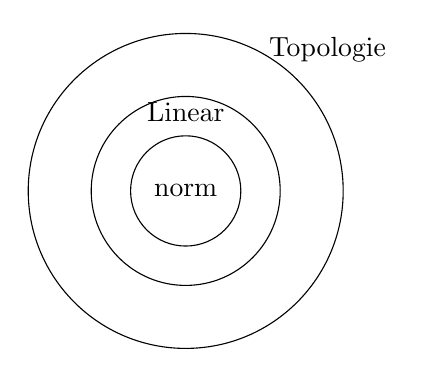
\begin{tikzpicture}
\draw (0,0) circle (2cm);
\draw (0,0) circle (1.2cm);
\draw (0,0) circle (0.7cm);
\node at (0,0) {norm};
\node at (0,1.0) {Linear};
\node at (1.8,1.8) {Topologie};
\end{tikzpicture}
\end{center}

\section{Unitary Space $(X, \langle \cdot, \cdot \rangle)$}

\begin{center}
Linear space on $\mathbb{K}$
\end{center}

$\langle \cdot, \cdot \rangle: X \times X \to \mathbb{K}$

\begin{enumerate}
\item[a)] $\forall x,y \in X \quad \langle x,y \rangle = \langle y, x \rangle$

\item[b)] $\forall y_1, y_2, \alpha, \beta, z \quad \langle \alpha x + \beta y_1, z \rangle$
\[ = \alpha \langle x, z \rangle + \beta \langle y_1, z \rangle \]

\item[c)] $\forall x \in X_{x \neq 0} \langle x, x \rangle > 0 \Rightarrow \langle x, x \rangle = 0 \Leftrightarrow x = 0$
\end{enumerate}

\vspace{0.5cm}
\textbf{Fakt:} $\|x\| = \sqrt{\langle x, x \rangle}$ is a norm

\vspace{0.5cm}
\textit{przykład:} $X = \mathbb{R}^n, \langle x, y \rangle = \sum x_i \cdot y_i$

$\|x\| = \left(\sum x_i^2\right)^{1/2}$

\section{Własności metryki przestrzeni}
\subsection{Nierówność Cauchy'ego-Schwarza}
$\forall x,y \in X \quad |\langle x,y \rangle| \leq \|x\| \cdot \|y\|$

$$\frac{\langle x,y \rangle}{\|x\| \cdot \|y\|} \in [-1,1]$$

\subsection{Tw. Pitagorasa $(x \perp y \Rightarrow \|x+y\|^2 = \|x\|^2 + \|y\|^2)$}
$$\|\sum x_k\|^2 = \sum \|x_k\|^2$$

\subsection{$f(y,y) = \arccos\left(\frac{\langle x,y \rangle}{\|x\| \cdot \|y\|}\right)$}

\vspace{0.3cm}
\textit{zbiory ciągłe}

\begin{enumerate}
\item $\forall \varepsilon > 0 \exists \delta > 0 \forall x_1, x_2 \in X \; d(x_1, x_2) < \varepsilon$
\item $\forall \varepsilon > 0 \exists \delta > 0 \forall x_1, m > 0 \; d(x_1, x_m) < \varepsilon$
\end{enumerate}

$(a) \Rightarrow (b) \quad (b) \Rightarrow (a)$ to przykład zupełnie

\vspace{0.3cm}
\textit{przykład}

$X = [0,1] \quad d(x,y) = |x-y| \quad x_n = \frac{1}{n}$

\end{document}
